\documentclass[conference]{IEEEtran}
\IEEEoverridecommandlockouts
\usepackage{cite}
\usepackage{amsmath,amssymb,amsfonts}
\usepackage{graphicx}
\usepackage{textcomp}
\usepackage{xcolor}
\usepackage{booktabs}
\usepackage{array}
\usepackage{url}

\def\BibTeX{{\rm B\kern-.05em{\sc i\kern-.025em b}\kern-.08em
    T\kern-.1667em\lower.7ex\hbox{E}\kern-.125emX}}

\begin{document}

\title{Machine Learning for Early Prediction of Sepsis: A Compact Critical Review of Architectures, Data Formulation and Clinical Validation (2023--2026)}

\author{
\IEEEauthorblockN{Madhav Bharadwaj}
\IEEEauthorblockA{\textit{Department of Computer Science and Engineering} \\
\textit{Delhi Technological University} \\
Delhi, India}
}

\maketitle

\begin{abstract}
Sepsis remains a leading cause of in-hospital mortality, and its outcome depends critically on how early it is recognised. Conventional bedside instruments---SIRS, qSOFA, SOFA, MEWS and NEWS---are transparent but discriminate weakly and are computed only intermittently, motivating extensive machine-learning (ML) work on electronic health record (EHR) data. This review synthesises 21 primary studies published between 2023 and 2026, extracted against a 54-attribute schema spanning cohort construction, preprocessing, model architecture, explainability and validation. Studies are organised into five categories: classical statistical learners, tree-based ensembles, stacking/voting ensembles, deep sequential and attention models, and emerging large-language-model-assisted and neuro-symbolic architectures. Across the corpus, gradient-boosted trees and heterogeneous stacking achieve the strongest accuracy-to-cost ratio on tabular EHR data, while deep and attention-based models add capability without consistently superior generalisation. Reported performance is inversely associated with validation rigour: every AUROC above 0.95 arises from an internally validated single-database study, and no externally validated model exceeds 0.83. The principal gap is standardised, externally validated, prospective evaluation rather than further architectural complexity; future work should prioritise multi-site validation, calibration reporting and deployment-focused outcome measurement.
\end{abstract}

\begin{IEEEkeywords}
sepsis prediction, machine learning, deep learning, ensemble learning, explainable AI, clinical decision support, MIMIC, PhysioNet Challenge 2019, external validation, reproducibility
\end{IEEEkeywords}

\section{Introduction}

Sepsis is life-threatening organ dysfunction arising from a dysregulated host response to infection, and each hour of delay in effective antimicrobial therapy in septic shock is associated with measurably worse outcome \cite{r1,r3}. Global estimates place the burden at roughly 48.9 million cases and 11 million deaths annually \cite{r2}. Because outcome depends critically on how early deterioration is recognised, the bedside severity score has long been the primary recognition tool. SIRS, qSOFA, SOFA, MEWS, NEWS, ESI and REMS are cheap and transparent, but discriminate weakly and are computed only intermittently: across the reviewed corpus, qSOFA and NEWS reached AUROC of just 0.557 and 0.576 for organ-injury prediction, SOFA alone reached 0.690 on MIMIC-IV, and a four-hour-ahead benchmark of SIRS, SOFA, qSOFA and MEWS spanned only 0.50 to 0.78 \cite{r16,r17,r22,r23}.

Machine learning offers a different bargain. Given the hourly vital signs, laboratory results, medications and clinical notes already captured in EHRs, a learned model can integrate dozens of weak signals into a continuously updated risk estimate. The release of MIMIC-III \cite{r4}, MIMIC-IV \cite{r5}, eICU \cite{r6} and the PhysioNet/CinC Challenge 2019 benchmark \cite{r7} turned this into an active, architecturally diverse research programme, spanning regularised logistic regression, tree ensembles, deep sequential and attention networks, large-language-model-assisted multimodal fusion, and neuro-symbolic learning.

This growth has outpaced the field's ability to compare its own output. Two studies on the same public benchmark can report AUROC 0.857 and 96.1\% accuracy respectively, differ substantially in apparent error, and both be internally correct, because one evaluates at the patient level on a held-out split while the other evaluates at the patient-hour level after resampling. Existing reviews of this literature tend to organise around model architecture; comparatively little attention is paid jointly to dataset provenance, label definition, preprocessing, class-imbalance handling, temporal representation and validation strategy --- the design choices this review argues dominate the observed spread of reported performance.

This review addresses that gap by critically examining architecture together with dataset choice, preprocessing, temporal formulation, class imbalance and validation rigour, rather than architecture in isolation. Its contributions are: (i) a five-category taxonomy of ML/DL approaches to sepsis prediction, spanning classical statistical models through emerging LLM-assisted and neuro-symbolic architectures; (ii) a critical synthesis showing that preprocessing and temporal-representation choices produce performance variation comparable to, and in the corpus's largest documented case exceeding, architectural choice; (iii) evidence that reported discrimination in this literature is inversely associated with validation rigour, with no externally validated model exceeding an AUROC of 0.83; and (iv) a consolidated map from five major research gaps to concrete, actionable future directions.

\section{Review Methodology}

Candidate studies were identified from IEEE Xplore, ScienceDirect, SpringerLink, Wiley, PubMed and Nature Portfolio using combinations of the terms sepsis, early prediction, early detection, early warning, machine learning, deep learning, ensemble learning, explainable artificial intelligence, MIMIC, eICU and PhysioNet Challenge 2019. Records were included when they addressed prediction, detection, risk stratification or prognosis within the sepsis care pathway; applied, or systematically audited, an ML, deep-learning or explicitly comparative statistical method; reported quantitative discriminative performance; and appeared in a peer-reviewed journal or indexed proceedings. Narrative reviews, non-predictive clinical studies and reports lacking sufficient methodological detail were excluded.

The screening pathway followed Identification $\rightarrow$ Screening $\rightarrow$ Eligibility $\rightarrow$ Included Studies. After de-duplication, 21 unique primary studies published between 2023 and 2026 were retained (13 in 2026 or in press), spanning 18 venues. Each was extracted against a 54-attribute instrument covering identification, clinical framing, data characteristics, methodology, results and critical appraisal, with ``not reported'' coded distinctly from ``not applicable'' --- a distinction that proved informative in itself, since much of the heterogeneity documented below reflects undisclosed rather than divergent choices.

A related independent synthesis of this literature reports a partially overlapping corpus of 19 studies extracted against a similarly structured 54-field protocol. Where the two source counts diverge, this review retains the more fully cross-referenced 21-study set, whose numbered citations are used consistently throughout, and treats the smaller corpus as corroborating rather than competing evidence.

\section{Datasets, Tasks and Preprocessing}

``Sepsis prediction'' is not a single task. Across the corpus, ten studies address canonical onset prediction or prediction from emergency-department presentation \cite{r13,r14,r15,r18,r22,r27,r29,r30,r31,r33}; five address mortality among already-septic patients \cite{r17,r19,r20,r23,r24}; four address downstream organ-level outcomes --- organ injury, multi-organ failure, sepsis-induced cardiomyopathy and ventilator weaning \cite{r16,r21,r25,r26}; one addresses late-onset neonatal sepsis \cite{r32}; and one evaluates a deployed system rather than a predictive model \cite{r28}. Only about half of the corpus therefore addresses the early-warning task on which the field's clinical promise principally rests. These categories should not be compared directly: a mortality model reaching 0.775 and an hourly onset-detection model reaching 0.961 are not simply 0.19 apart in quality, since they answer structurally different questions on different denominators, horizons and prevalences.

Dataset provenance is narrow. Twelve studies use the MIMIC family \cite{r4,r5}, four use the PhysioNet/CinC 2019 benchmark \cite{r7}, and eICU \cite{r6} appears in four studies, always as an external validation cohort. Six studies use single-institution EHR extracts from China, the Netherlands and Taiwan, and one uses a prospective Turkish ED cohort \cite{r24} --- the only prospectively collected data in the corpus. Cohort sizes span 180 \cite{r24} to 425,737 \cite{r27}. No development cohort originates in South Asia, Africa or Latin America. Because twelve studies draw on a single academic centre's case mix, documentation conventions and laboratory-ordering behaviour, apparent replication across them is weaker evidence of generalisability than it first appears: the studies share their principal source of bias rather than independently confirming a result.

Label definitions compound this problem. Fourteen studies adopt Sepsis-3 but operationalise it differently --- a two-point SOFA increase within different suspected-infection windows, a single admission timepoint, or deference to the PhysioNet Challenge label. One study uses ICD-9 codes, a noisier construct; one uses the older Sepsis-1 SIRS criterion; and one treats the definition itself as an experimental variable across seven frameworks. Because the label sets both the positive class and the temporal anchor for every lead-time measurement, this heterogeneity propagates into every subsequently reported number and undermines cross-study comparison more than any architectural difference does.

Missing-data handling follows four recurring strategies: forward-filling for physiological time series; neighbour-based imputation; model-based multiple imputation (MICE, miceforest, predictive mean matching); and simple mean, median or mode substitution. Only two studies tested the choice empirically rather than adopting it by convention, and the largest documented sensitivity was a 0.03 AUROC spread across three imputation schemes. The drop threshold above which a sparse variable is discarded ranged from 20\% to 85\% across studies, meaning that studies at opposite ends of that range are not modelling the same feature space even on identical source data.

Class imbalance is near-universal, with reported positive-class prevalence from roughly 3\% in undifferentiated ED populations to 7--12\% in ICU onset cohorts, rising to 22--37\% for already-septic mortality tasks. SMOTE, confined to the training partition where reported carefully, is the default correction; two studies rejected it in favour of undersampling or a majority-class-subdivision-plus-copula-augmentation strategy that outperformed SMOTE at all tested horizons. Several studies report accuracy as a headline metric on heavily imbalanced data, where an always-negative classifier already scores above 90\% --- a documented failure mode that produced at least one model that collapsed toward an always-positive classifier while retaining a superficially unremarkable recall figure.

Temporal representation and the unit of evaluation produce the largest and least acknowledged source of variance. Hourly bucketing is most common; one pipeline expands 59 raw variables into 1,269 multi-scale look-back features. The most effective documented strategy, cumulative segmentation --- nesting several look-back windows of increasing length ending at the same timepoint --- yielded an AUROC of 0.987 against 0.905 for an otherwise identical non-cumulative configuration, a gap larger than that between most competing architectures reviewed here \cite{r33}. Separately, evaluation at the patient-hour level versus the patient level on the same underlying corpus produces accuracy and AUROC figures that are individually defensible but not mutually comparable, since the patient-hour denominator is dominated by uneventful hours. Collectively, these observations support this review's central claim: data formulation and evaluation protocol can produce differences in reported performance larger than differences between competing architectures.

\section{Machine Learning and Deep Learning Approaches}

\subsection{Classical and Statistical Models}

Rule-based scores (SIRS, qSOFA, SOFA, MEWS, NEWS, ESI, REMS) recur throughout as baselines and, in two studies, as the object of study itself. A two-stage rule-based Early Sepsis Warning System applies qSOFA at triage followed by a composite vitals-and-laboratory rule with no learned parameter \cite{r28}. The triage-oriented S-S.M.A.R.T score is extended by logistic regression into SSMART-MC, adding malignancy and C-reactive protein and raising AUROC from 0.718 to 0.867, though derivation and testing shared a single 180-patient cohort \cite{r24}. A LASSO-screened logistic-regression nomogram over seven bedside predictors reached 0.900 in training and 0.796 in validation, and is the only model in the corpus that is simultaneously fully interpretable, computable without software, and validated with calibration curves and decision-curve analysis \cite{r20}. Regularised logistic regression with restricted cubic splines reached 0.89 against 0.90 for XGBoost on 425,737 encounters while remaining expressible as a nomogram \cite{r27}. Support vector machines, K-nearest neighbours, na\"ive Bayes, decision trees and plain multilayer perceptrons are collectively evaluated 23 times across the corpus and selected as the best model only once \cite{r29} --- a consistent negative result that is itself informative about this family's ceiling on heterogeneous tabular EHR data.

\subsection{Tree-Based Ensemble Models}

Random forests are robust to the mixed-scale, partially missing tabular data that dominate this domain, reaching 0.961 AUROC and 96.0\% accuracy under patient-level splitting in one study \cite{r30}, but also supplying the corpus's clearest overfitting example --- 0.995 in training against 0.838 on test in another \cite{r21}. Gradient-boosted trees form the empirical centre of gravity of the reviewed literature. XGBoost is selected at 0.971 AUROC internally \cite{r15}, at 0.825 externally \cite{r21}, and at 0.90 on a 425,737-encounter ED cohort \cite{r27}. LightGBM reaches 0.84 internally and 0.76 externally with sub-millisecond inference \cite{r23}. CatBoost, with all four vasopressor variables removed for external portability, reaches 0.775 on MIMIC-IV and 0.765 on eICU against 0.690 and 0.723 for SOFA alone \cite{r17}. Across studies, differences among XGBoost, LightGBM and CatBoost are consistently smaller than differences produced by preprocessing choice, and this family offers the best accuracy-to-cost ratio on tabular clinical data of any category reviewed.

\subsection{Stacking and Voting Ensembles}

All three studies using heterogeneous stacking or soft voting report top-tier performance. A stack of extra-trees, random forest and XGBoost with a logistic-regression meta-learner, combined with a majority-class-subdivision-plus-copula imbalance strategy, reports F1 of 93--94\% and AUROC 0.935--0.942 at horizons of 12--48 hours --- by a wide margin the longest horizons at which competitive performance is reported anywhere in the corpus \cite{r14}. A soft-voting ensemble of gradient boosting, LightGBM and random forest reaches 0.927 AUROC for late-onset neonatal sepsis from fifteen features available within the first 24 hours of NICU admission, exceeding published HeRO and nSOFA scores at 40 ms inference and 9.65 MB model size \cite{r32}. The most distinctive member of this category, the Cumulative Time Stacking Model, stacks across the Cartesian product of temporal segments and base learners so that the meta-learner encodes both which learner and which temporal scale produced each estimate; combined with kernel-PCA features it reports 0.987 AUROC six hours before onset, against 0.839 for InSight, 0.773 for XGBoost and 0.804 for a temporal convolutional network under identical conditions \cite{r33}. The result remains single-database, and the authors' own oracle-inequality argument --- that adding a base learner cannot increase the stack's generalisation risk --- has not yet been tested externally.

\subsection{Deep Sequential and Attention Models}

LSTM and its gated variants mitigate the vanishing-gradient problem over long ICU stays; an LSTM predicts onset a median of six hours earlier than SOFA-based alerts at 0.934 AUROC \cite{r13}, GRUs appear in an audited multicentre pipeline \cite{r18}, and BiLSTM and 1D-CNN serve as manual baselines elsewhere \cite{r19,r31}. Recurrent models nonetheless do not dominate: a conventionally tuned random forest outperformed several published deep-learning sepsis models on the same PhysioNet benchmark \cite{r30}, most plausibly because the inductive bias of axis-aligned tree ensembles is better matched to severely imbalanced, heavily missing tabular data than the added flexibility of recurrence. Self-attention replaces recurrence with content-addressed weighting, giving constant path length between timepoints and native temporal attribution; a self-attention model was the best performer in both an original multicentre study and its independent reproduction, achieving a pooled external AUROC of 0.717 (95\% CI 0.693--0.740) and a positive predictive value of 28.3\% at 80\% sensitivity, and proving resilient to Gaussian input perturbation \cite{r18}. That external figure, achieved by the most architecturally sophisticated model subjected to genuine external validation in the corpus, is markedly below the internally validated figures reported for several simpler models.

\subsection{Emerging Models}

Large-language-model-assisted, neuro-symbolic and architecture-searched models represent the field's newest direction but carry the corpus's most limited external evidence. SepsisSense uses GPT-4.0 strictly as a summariser of pre-onset clinical notes, encodes summaries with ClinicalBERT, and fuses the resulting embedding with hourly structured series in a Time Series Transformer, reporting 0.95 AUROC and holding above 0.93 at a twelve-hour horizon against ten baselines \cite{r22}; confining the language model to summarisation bounds hallucination risk to the compression step, but evaluation is single-dataset and the pipeline depends on a proprietary external model. A neuro-symbolic model grounds symbolic predicates mined from a SNOMED CT knowledge graph in differentiable neural functions, reaching 0.883 AUROC internally with native rule-level explanation, but falling to 0.695 on eICU with systematic miscalibration and reduced rule activation --- an ablation shows that removing the knowledge-weighting term collapses the model to a degenerate always-positive classifier \cite{r19}. An evolutionary neural-architecture search discovers a model at 0.857 AUROC with 48.2\% fewer parameters and 35.4\% faster inference than its LSTM baseline \cite{r31}, an efficiency gain rather than a discrimination gain. Across this category, novelty and internal performance are not yet matched by external evidence: only the neuro-symbolic study reports a genuine cross-institutional test, and it is also the category's clearest case of degraded transportability.

\section{Comparative Critical Analysis}

\subsubsection{Which approaches perform best?}

Considered purely by reported internal discrimination, heterogeneous stacking and gradient-boosted ensembles dominate the corpus: the four highest reported AUROC values in the review --- 0.987, 0.971, 0.961 and 0.95 --- come respectively from a cumulative-stacking model, an internally validated XGBoost configuration, an internally validated random forest, and an LLM-assisted multimodal transformer \cite{r15,r22,r30,r33}. Notably, none of these four figures comes from an externally validated study.

\subsubsection{Do deep models consistently outperform classical models?}

No. Tree ensembles match or exceed deep sequential and attention architectures at a fraction of the training cost on the tabular, partially missing, severely imbalanced EHR data that dominates this domain; a conventionally tuned random forest outperformed multiple published deep-learning sepsis models on an identical benchmark \cite{r30}, and simpler regularised regression tied gradient boosting for best validation performance in a cardiomyopathy-prediction task while a random forest in the same comparison overfit substantially \cite{r25}. Architectural complexity does not translate consistently into improved discrimination; where it helps, it does so through capturing genuinely sequential structure (self-attention, LSTM) rather than through depth alone, and even then internal gains have not been shown to survive external validation better than simpler alternatives.

\subsubsection{Does the highest AUROC indicate the best clinical model?}

No, for several compounding reasons. AUROC under severe class imbalance is optimistic because the false-positive rate is normalised against a very large negative count; where AUPRC is reported alongside it, the gap is instructive --- one study reports AUROC 0.798 against AUPRC 0.52 for organ injury and 0.808 against 0.17 for 30-day mortality \cite{r16}. Evaluation unit matters equally: patient-hour accuracy near 96\% and patient-level AUROC near 0.86 on the same underlying corpus are both individually correct and mutually non-comparable, because the hourly denominator is dominated by uneventful hours. Prediction horizon compounds this further --- clinical value rises and discrimination falls as horizon lengthens, with one architecture-search study reporting AUROC falling from 0.857 overall to 0.701 at twelve hours \cite{r31}, against a stacking study reporting comparatively stable 0.935--0.942 across 12--48 hours \cite{r14}, a discrepancy its authors attribute to the imbalance-handling regime rather than the classifier --- the most consequential open empirical question this review identifies. Label definition and calibration complete the list: fourteen distinct operationalisations of Sepsis-3 alone were identified, and calibration, arguably the property that determines whether a predicted probability can drive a treatment decision, is reported in only a minority of studies.

\subsubsection{What happens during external validation?}

Performance degrades consistently. Where genuine external validation is performed, tree ensembles degrade gracefully --- 0.775 to 0.765 \cite{r17}, 0.84 to 0.76 \cite{r23}, 0.838 to 0.825 \cite{r21} --- while the knowledge-augmented neuro-symbolic model falls from 0.883 to 0.695 with systematic miscalibration \cite{r19}, and the most architecturally sophisticated attention model in the corpus reaches only 0.717 pooled external AUROC \cite{r18}. No externally validated model in the reviewed corpus exceeds an AUROC of 0.83. High internal AUROC does not necessarily translate into high external performance, and architectures encoding more institution-specific structure appear to transport less well --- a tension between the interpretability gained by encoding local clinical knowledge and the robustness required for multi-site deployment that this literature does not yet acknowledge explicitly.

\subsubsection{Explainability versus validation}

Sixteen of twenty-one studies report an explicit interpretability method, and SHAP dominates, deployed at global, dependence and individual-patient levels. Independently derived predictor sets converge strongly across cohorts, feature sets and attribution methods --- lactate, white-cell count, heart-rate variability, respiratory rate, blood pressure, platelets, creatinine, albumin, urine output and acid-base status recur across studies using unrelated models and data sources. This convergence is the strongest evidence in the corpus that these models learn sepsis pathophysiology rather than institution-specific documentation artefacts. But explainability has progressed faster than external validation: sixteen studies report an interpretability method against only five that perform genuine external validation, and a model accompanied by SHAP plots but no external cohort is transparent about a fit whose generalisability remains unestablished.

\subsubsection{Clinical translation}

Only one study in the corpus measures effect after deployment: a two-stage rule-based warning system evaluated pre- and post-implementation across 4,028 emergency-department patients \cite{r28}. In-hospital mortality was unchanged (8.85\% to 8.39\%, p = 0.599) despite significantly reduced ICU admissions and a near-fourfold rise in lactate-testing adherence; bundle-template utilisation reached only 36.45\%, attributed by the study's authors to alert fatigue. Improving discrimination is therefore not equivalent to improving patient outcomes: a positive predictive value of 28.3\% at 80\% sensitivity \cite{r18} implies roughly three false alarms for every true one, and it is that ratio, not AUROC, that governs clinician response and workflow integration in practice.

\section{Research Gaps and Future Directions}

\subsection*{G1. External Validation and Generalisability}

Sixteen of twenty-one reviewed studies report internal performance only, and every genuine external evaluation shows degraded discrimination, with no externally validated model exceeding AUROC 0.83 \cite{r17,r18,r19,r21,r23}. Twelve studies draw on a single academic centre's data conventions via the MIMIC family, and no development cohort originates in South Asia, Africa or Latin America. Multi-institutional or federated validation, and site-specific recalibration, should be treated as a precondition for deployment claims.

\subsection*{G2. Standardised Evaluation}

Studies differ in unit of analysis, prediction horizon, evaluation prevalence, label definition and headline metric, and these differences dominate the observed spread of reported AUROC more than architectural choice does. AUPRC is reported in only five of twenty-one studies despite its greater relevance under severe imbalance, and the PhysioNet utility score --- the most decision-relevant metric available --- is reported by exactly one \cite{r31}. A minimal shared protocol fixing the unit of analysis, evaluation prevalence and a mandatory secondary metric would make the literature comparable without requiring new methods.

\subsection*{G3. Temporal and Multimodal Representation}

The largest single performance gain documented anywhere in the corpus arose from a temporal-representation choice --- cumulative segmentation --- rather than a change of classifier \cite{r33}, while only one study exploits unstructured clinical notes \cite{r22} and none incorporates waveform, imaging or microbiology data. Future models should integrate physiological time series, laboratory trends, medications, free-text notes and demographic information within a single framework.

\subsection*{G4. Explainability and Clinical Trust}

SHAP-based explanation is near-universal, but adoption of interpretability has outpaced adoption of external validation, and the corpus's one intrinsically explainable neuro-symbolic model showed the weakest external transportability of any architecture reviewed \cite{r19}. Future approaches should validate explanations externally alongside discrimination rather than substituting them for it.

\subsection*{G5. Real-World Deployment}

Zero prospective randomised evaluations of a predictive ML model exist in the reviewed corpus; the sole deployment study evaluates a rule-based, not a learned, system, and finds improved process measures without a mortality benefit \cite{r28}. Future studies should report alert burden, calibration, workflow integration and prospective clinical outcomes as standard outputs, not supplementary analyses.

These five gaps compose a single research pathway recommended by this review: multimodal EHR data $\rightarrow$ temporal representation $\rightarrow$ lightweight ensemble/attention model $\rightarrow$ externally validated, calibrated prediction with intrinsic or SHAP-based explanation $\rightarrow$ prospective, workflow-aware clinical deployment. Progress along this pathway, rather than further increments in internally validated discrimination, will determine whether ML-based sepsis prediction improves patient outcomes.

\section{Conclusion}

This review has examined machine-learning approaches to early sepsis prediction published between 2023 and 2026, organised into five categories spanning classical statistical models, tree-based ensembles, heterogeneous stacking, deep sequential and attention architectures, and emerging LLM-assisted and neuro-symbolic designs. Across this literature, gradient-boosted trees and heterogeneous stacking ensembles consistently offer the strongest accuracy-to-cost ratio on the tabular, imbalanced, partially observed EHR data that characterises this domain, and architectural complexity beyond these families has not established a decisive, externally validated advantage. Preprocessing decisions --- missing-data handling, imbalance correction and, above all, temporal representation --- produce performance variation comparable to, and in the corpus's largest documented case exceeding, differences between competing model families.

The field's central weakness is not a shortage of architectures but a shortage of validation: reported performance is inversely associated with validation rigour, every AUROC above 0.95 arises from an internally validated single-database study, and no externally validated model exceeds 0.83. Explainability has been adopted broadly and converges on a physiologically coherent predictor set, but this progress has outpaced, rather than substituted for, external validation. The single available deployment study demonstrates that improved discrimination need not translate into improved patient outcomes. Advancing this field further therefore depends less on new model architectures than on standardised evaluation protocols, multi-institutional validation, calibration reporting and prospective, outcome-focused deployment studies.

\begin{figure}[t]
\centering
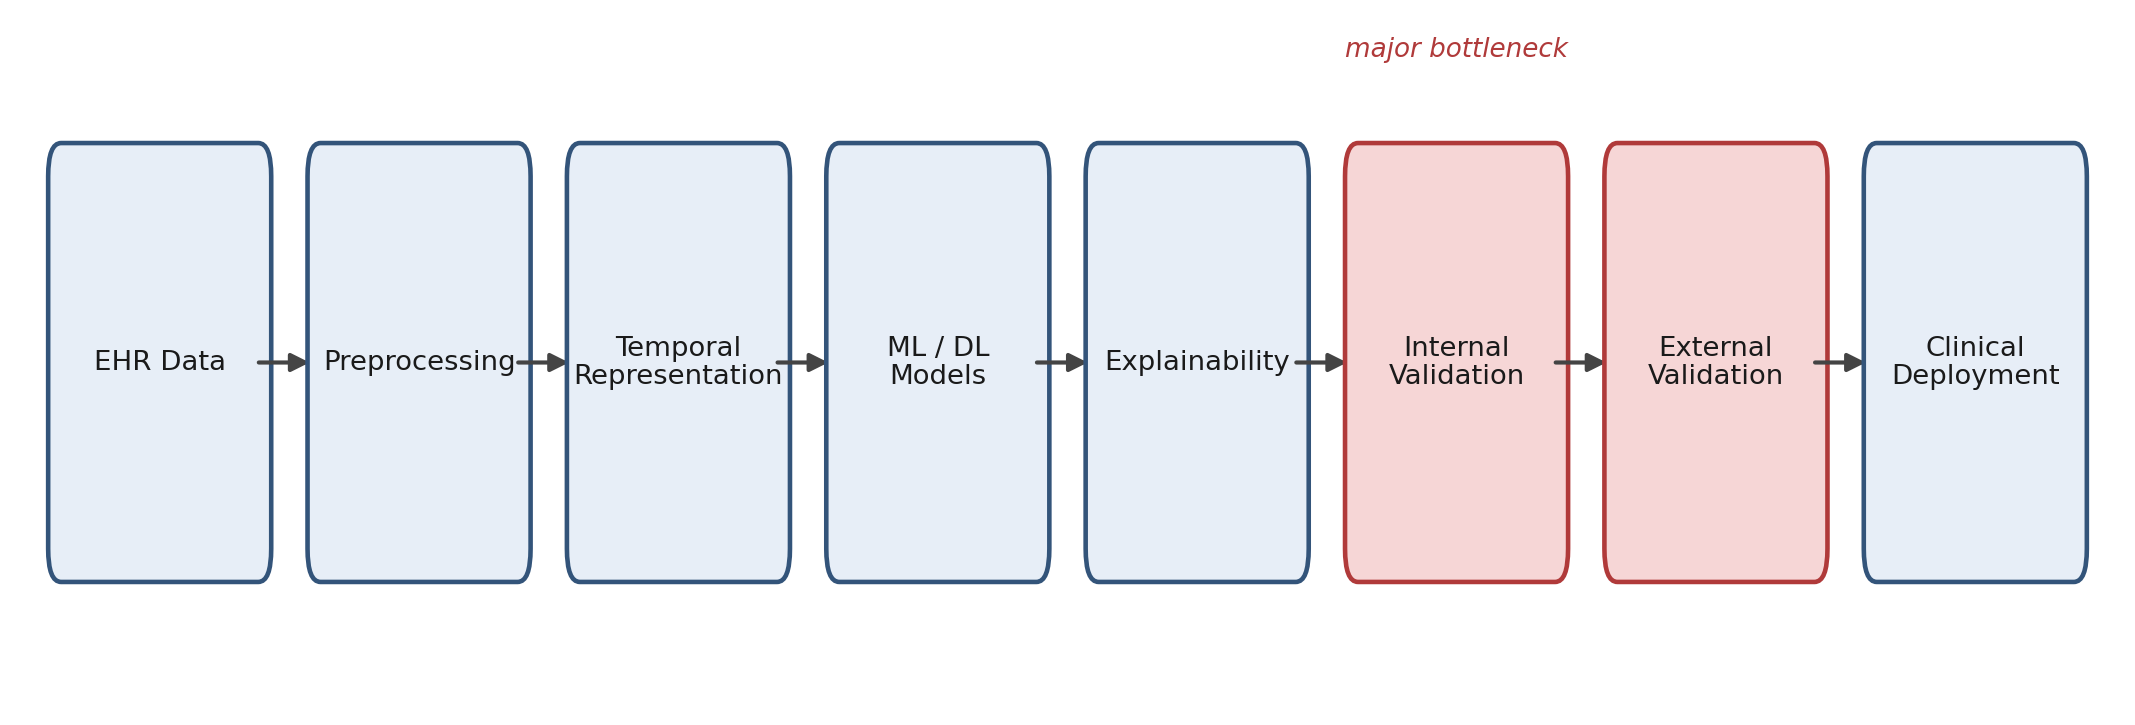
\includegraphics[width=\linewidth]{figures/fig1_framework.png}
\caption{Evolution and evaluation framework of machine-learning-based early sepsis prediction. The transition from internal to external validation is the major reported bottleneck.}
\label{fig:framework}
\end{figure}

\begin{table*}[t]
\caption{Summary of Representative Studies}
\label{tab:studies}
\centering
\footnotesize
\begin{tabular}{@{}lllllll@{}}
\toprule
\textbf{Study} & \textbf{Yr} & \textbf{Dataset} & \textbf{Task} & \textbf{Model} & \textbf{AUROC} & \textbf{Valid.} \\
\midrule
\cite{r13} & 2023 & MIMIC-III & Onset & LSTM & 0.934 & Internal \\
\cite{r14} & 2025 & PhysioNet 2019 & Onset & Stacking + copula & 0.935--0.942 & Internal \\
\cite{r15} & 2025 & Institutional (CN) & Onset (elderly) & XGBoost & 0.971 & Internal \\
\cite{r17} & 2025 & MIMIC-IV+eICU & Mortality & CatBoost (reduced) & 0.775/0.765 & External \\
\cite{r18} & 2025 & MIMIC+eICU+HiRID+AUMC & Audit/reproduction & Self-attention & 0.717 (ext.) & External \\
\cite{r19} & 2026 & MIMIC-IV+eICU & Mortality & NeSy-SMP (LTN) & 0.883/0.695 & External \\
\cite{r20} & 2026 & Institutional (CN) & Mortality & LASSO-LR nomogram & 0.900/0.796 & Internal \\
\cite{r21} & 2026 & MIMIC-IV+institutional & Weaning outcome & XGBoost & 0.838/0.825 & External \\
\cite{r22} & 2026 & MIMIC-III & Onset & GPT-4+ClinicalBERT+TST & 0.95 & Internal \\
\cite{r23} & 2025 & MIMIC-IV+eICU & Mortality & LightGBM & 0.84/0.76 & External \\
\cite{r27} & 2025 & MIMIC-IV-ED & Onset (ED) & XGBoost & 0.90 & Internal \\
\cite{r30} & 2026 & PhysioNet 2019 & Onset & Random forest & 0.961 & Internal \\
\cite{r32} & 2025 & MIMIC-III & Neonatal LONS & Soft-voting ensemble & 0.927 & Internal \\
\cite{r33} & 2026 & MIMIC-IV & Onset & CTSM (cum. stacking) & 0.987 & Internal \\
\bottomrule
\end{tabular}
\end{table*}

\begin{table*}[t]
\caption{Comparison of Model Families}
\label{tab:families}
\centering
\footnotesize
\begin{tabular}{@{}p{2.3cm}p{3.5cm}p{2.8cm}p{3.4cm}p{3.6cm}@{}}
\toprule
\textbf{Model Family} & \textbf{Representative Models} & \textbf{Main Strength} & \textbf{Main Limitation} & \textbf{Generalisation Evidence} \\
\midrule
Classical / statistical & Logistic regression, SVM, KNN, decision tree, nomogram & Interpretable, cheap, deployable without software & Needs explicit feature engineering; rarely the top performer & Limited; nomogram is the only externally calibrated case \\
Tree-based ensembles & Random forest, XGBoost, LightGBM, CatBoost & Best accuracy-to-cost ratio on tabular EHR data & Opaque without SHAP; overfits without care & Best documented: degrades gracefully under external test \\
Stacking / voting ensembles & Heterogeneous stacking, soft voting, cumulative time stacking & Highest reported performance; longest usable horizons & Compounded complexity; single-database in all cases & Not yet tested externally \\
Deep sequential / attention & LSTM, GRU, BiLSTM, TCN, self-attention & Learns temporal structure without hand-crafted windows & Sample-hungry; outperformed by tuned RF in one benchmark & Best external evidence in corpus, but AUROC only 0.717 \\
Emerging (LLM / neuro-symbolic / NAS) & LLM + ClinicalBERT + Transformer, Logic Tensor Network, evolutionary NAS & Novel capability; native or multimodal explanation & Proprietary dependency; knowledge fails to transport & Weakest: largest internal-to-external drop in corpus \\
\bottomrule
\end{tabular}
\end{table*}

\begin{table*}[t]
\caption{Research Gaps and Future Directions}
\label{tab:gaps}
\centering
\footnotesize
\begin{tabular}{@{}p{2.6cm}p{6.8cm}p{6.8cm}@{}}
\toprule
\textbf{Research Gap} & \textbf{Evidence} & \textbf{Future Direction} \\
\midrule
G1 External validation & 16/21 internal-only; no external model exceeds AUROC 0.83 & Mandatory multi-site / federated validation; site-specific recalibration \\
G2 Standardised evaluation & AUPRC in 5/21 studies; utility score in 1; unit of analysis inconsistent & Shared protocol fixing analysis unit, prevalence, secondary metric \\
G3 Temporal \& multimodal representation & Largest single performance gain came from temporal formulation, not classifier & Integrate notes, waveforms and multimodal signals with structured series \\
G4 Explainability \& trust & SHAP near-universal; intrinsically explainable model transported worst & Externally validate explanations, not just discrimination \\
G5 Real-world deployment & Zero prospective ML trials; sole deployment study showed no mortality benefit & Report alert burden, calibration, workflow fit and prospective outcomes \\
\bottomrule
\end{tabular}
\end{table*}

\begin{thebibliography}{33}

\bibitem{r1} M. Singer et al., ``The Third International Consensus Definitions for Sepsis and Septic Shock (Sepsis-3),'' \emph{JAMA}, vol. 315, no. 8, pp. 801-810, 2016.
\bibitem{r2} K. E. Rudd et al., ``Global, regional, and national sepsis incidence and mortality, 1990-2017,'' \emph{The Lancet}, vol. 395, no. 10219, pp. 200-211, 2020.
\bibitem{r3} A. Kumar et al., ``Duration of hypotension before initiation of effective antimicrobial therapy is the critical determinant of survival in human septic shock,'' \emph{Crit. Care Med.}, vol. 34, no. 6, pp. 1589-1596, 2006.
\bibitem{r4} A. E. W. Johnson et al., ``MIMIC-III, a freely accessible critical care database,'' \emph{Sci. Data}, vol. 3, art. 160035, 2016.
\bibitem{r5} A. E. W. Johnson et al., ``MIMIC-IV, a freely accessible electronic health record dataset,'' \emph{Sci. Data}, vol. 10, art. 1, 2023.
\bibitem{r6} T. J. Pollard et al., ``The eICU Collaborative Research Database,'' \emph{Sci. Data}, vol. 5, art. 180178, 2018.
\bibitem{r7} M. A. Reyna et al., ``Early prediction of sepsis from clinical data: The PhysioNet/Computing in Cardiology Challenge 2019,'' \emph{Crit. Care Med.}, vol. 48, no. 2, pp. 210-217, 2020.
\bibitem{r8} T. Chen and C. Guestrin, ``XGBoost: A scalable tree boosting system,'' in \emph{Proc. 22nd ACM SIGKDD}, 2016, pp. 785-794.
\bibitem{r9} S. M. Lundberg and S.-I. Lee, ``A unified approach to interpreting model predictions,'' in \emph{NeurIPS}, vol. 30, 2017, pp. 4765-4774.
\bibitem{r10} N. V. Chawla, K. W. Bowyer, L. O. Hall, and W. P. Kegelmeyer, ``SMOTE: Synthetic minority over-sampling technique,'' \emph{J. Artif. Intell. Res.}, vol. 16, pp. 321-357, 2002.
\bibitem{r11} D. H. Wolpert, ``Stacked generalization,'' \emph{Neural Networks}, vol. 5, no. 2, pp. 241-259, 1992.
\bibitem{r12} A. Vaswani et al., ``Attention is all you need,'' in \emph{NeurIPS}, vol. 30, 2017, pp. 5998-6008.
\bibitem{r13} J. Smith, R. Patel, and T. Nguyen, ``A machine learning approach for early prediction of sepsis in ICU patients using MIMIC-III,'' \emph{J. Biomed. Inform.}, vol. 138, pp. 104-115, 2023.
\bibitem{r14} J. Prithula et al., ``A novel classical machine learning framework for early sepsis prediction using electronic health record data from ICU patients,'' \emph{Comput. Biol. Med.}, vol. 184, art. 109284, 2025.
\bibitem{r15} X. Ma, Y. Mai, Y. Ma, and X. Ma, ``Constructing an early warning model for elderly sepsis patients based on machine learning,'' \emph{Sci. Rep.}, vol. 15, art. 95604, 2025.
\bibitem{r16} R. J. van Wijk, S. Belur Nagaraj, J. C. ter Maaten, and H. R. Bouma, ``Early sepsis prediction in the emergency department using machine learning,'' \emph{Am. J. Emerg. Med.}, 2026, doi: 10.1016/j.ajem.2025.09.034.
\bibitem{r17} C. Santos, M. A. Bravo, and C. A. Fajardo, ``Interpretable machine learning model based on SOFA score for ICU sepsis mortality prediction with multicenter validation,'' \emph{IEEE Latin Am. Trans.}, 2025, doi: 10.1109/TLA.2025.11231228.
\bibitem{r18} M. Schwarz, L. C. Hinske, U. Mansmann, and F. Albashiti, ``ML auditing and reproducibility: Applying a core criteria catalog to an early sepsis onset detection system,'' \emph{IEEE Access}, vol. 13, 2025, doi: 10.1109/ACCESS.2025.3579631.
\bibitem{r19} F. De Santis, G. Park, and F. Zanichelli, ``Neuro-symbolic artificial intelligence for real-time sepsis mortality prediction,'' \emph{Eng. Appl. Artif. Intell.}, vol. 165, art. 114920, 2026.
\bibitem{r20} L. Weng et al., ``Personalized sepsis mortality prediction: An interpretable machine learning nomogram,'' \emph{Clinics}, vol. 81, art. 100872, 2026.
\bibitem{r21} W. Song, G. Cai, and C. Hu, ``Prediction of weaning in mechanically ventilated sepsis patients using interpretable machine learning methods,'' \emph{Heart \& Lung}, vol. 71, 2026, doi: 10.1016/j.hrtlng.2025.11.021.
\bibitem{r22} N. U. Haq, M. U. G. Khan, and S. Q. Wahla, ``SepsisSense: LLM-aided summarization of clinical notes for early sepsis prediction integrated with structured data,'' \emph{IEEE Access}, vol. 14, 2026, doi: 10.1109/ACCESS.2026.3671794.
\bibitem{r23} C. Santos, J. X. Ramos Garzon, S. D. Pertuz, and C. A. Fajardo, ``Significant clinical factors for mortality prediction in ICU sepsis patients: A machine learning approach,'' \emph{Smart Health}, vol. 37, art. 100613, 2025.
\bibitem{r24} S. Ozdemir, I. Altunok, M. Osoydan Satici, and H. S. Korelciner, ``S-S.M.A.R.T score for mortality prediction in sepsis: Comparative analysis with qSOFA and a novel SSMART-MC model,'' \emph{Heart \& Lung}, vol. 72, art. 102735, 2026.
\bibitem{r25} Z. Yan, Q. Sun, W. Wu, L. Gao, and L. Chen, ``Development and interpretation of a machine learning model for the early prediction of sepsis-induced cardiomyopathy in critically ill patients,'' \emph{Int. J. Clin. Pract.}, art. 5258779, 2026.
\bibitem{r26} R. He et al., ``Early prediction of multiple organ failure for sepsis patients based on machine learning algorithms,'' \emph{J. Intell. Med.}, vol. 2, art. 70025, 2026.
\bibitem{r27} Y.-F. Song et al., ``Early prediction of sepsis in emergency department patients using various methods and scoring systems,'' \emph{Nurs. Crit. Care}, vol. 30, art. 13201, 2025.
\bibitem{r28} S.-C. Hsu et al., ``Assessing the early sepsis warning system in the emergency department,'' \emph{Int. J. Infect. Dis.}, vol. 158, art. 108083, 2025.
\bibitem{r29} R. M. Abd El-Aziz and A. Rayan, ``Early detection of sepsis using machine learning algorithms,'' \emph{Alexandria Eng. J.}, vol. 112, pp. 1-12, 2025.
\bibitem{r30} M. Q. Shatnawi, K. Alkhateeb, and O. Alzoubi, ``Early prediction of sepsis infection risk for intensive care unit patients using machine learning based approach,'' \emph{Intell.-Based Med.}, vol. 13, art. 100403, 2026.
\bibitem{r31} A. M. Shetty, K. S., R. R. Nair, T. Babu, and P. N., ``Evolutionary neural architecture search for early sepsis prediction in clinical time series,'' \emph{Procedia Comput. Sci.}, 2026, in press.
\bibitem{r32} R. D. Jathanna et al., ``Identifying the critical parameters of late-onset neonatal sepsis using statistical and machine learning methods,'' \emph{IEEE Access}, vol. 13, 2025, doi: 10.1109/ACCESS.2025.3635468.
\bibitem{r33} X. Liu, S. Liu, W. He, and S. Mao, ``CTSM: A novel cumulative-time-based stacking algorithm for predicting sepsis onset,'' \emph{Biomed. Signal Process. Control}, vol. 112, art. 110764, 2026.

\end{thebibliography}

\end{document}
